\begin{tikzpicture}
  \pgfmathsetseed{3}
  \node at (0,0) {
    \begin{tikzpicture}[thick]
    \draw plot [smooth cycle, samples=8,domain={1:8}] (\x*360/8+5*rnd:0.5cm+1.5cm*rnd) node at (0,0) {$\mathcal{R}$};
    \end{tikzpicture}
  };
  %\path[->,thick] (1.75,0) edge [bend left] node[above,yshift=0.125cm] {$\alpha$-inference} (3.25,0);
  \path[->,thick] (1.75,0) edge [bend left] node[above,align=center,yshift=0.125cm] {auxiliary\\inference} (3.25,0);
  \pgfmathsetseed{11}
  \node at (5,0) {
    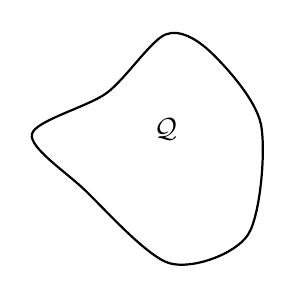
\begin{tikzpicture}[thick]
    \draw plot [smooth cycle, samples=8,domain={1:8}] (\x*360/8+5*rnd:0.5cm+1.5cm*rnd) node at (0,0) {$\mathcal{Q}$};
    \end{tikzpicture}
  };
  \path[->,thick] (6.75,0) edge [bend left] node[above,align=center,yshift=0.125cm] {variational\\inference} (8.25,0);
  \pgfmathsetseed{9}
  \node at (10,0) {
    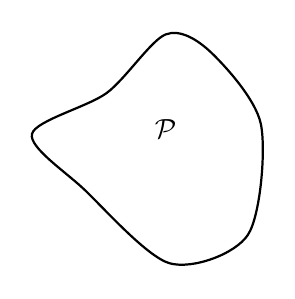
\begin{tikzpicture}[thick]
    \draw plot [smooth cycle, samples=8,domain={1:8}] (\x*360/8+5*rnd:0.5cm+1.5cm*rnd) node at (0,0) {$\mathcal{P}$};
    \end{tikzpicture}
  };
\end{tikzpicture}
